\let\negmedspace\undefined
\let\negthickspace\undefined
\documentclass[journal]{IEEEtran}
\usepackage[a5paper, margin=10mm, onecolumn]{geometry}
%\usepackage{lmodern} % Ensure lmodern is loaded for pdflatex
\usepackage{tfrupee} % Include tfrupee package

\setlength{\headheight}{1cm} % Set the height of the header box
\setlength{\headsep}{0mm}     % Set the distance between the header box and the top of the text

\usepackage{gvv-book}
\usepackage{gvv}
\usepackage{cite}
\usepackage{amsmath,amssymb,amsfonts,amsthm}
\usepackage{algorithmic}
\usepackage{graphicx}
\usepackage{textcomp}
\usepackage{xcolor}
\usepackage{txfonts}
\usepackage{listings}
\usepackage{enumitem}
\usepackage{mathtools}
\usepackage{gensymb}
\usepackage{comment}
\usepackage[breaklinks=true]{hyperref}
\usepackage{tkz-euclide} 
\usepackage{listings}
% \usepackage{gvv}                                        
\def\inputGnumericTable{}                                 
\usepackage[latin1]{inputenc}                                
\usepackage{color}                                            
\usepackage{array}                                            
\usepackage{longtable}                                       
\usepackage{calc}                                             
\usepackage{multirow}                                         
\usepackage{hhline}                                           
\usepackage{ifthen}                                           
\usepackage{lscape}
\begin{document}

\bibliographystyle{IEEEtran}
\vspace{3cm}

\title{4.3.50}
\author{EE25BTECH11060 - V.Namaswi}
% \maketitle
% \newpage
% \bigskip
{\let\newpage\relax\maketitle}
\renewcommand{\thefigure}{\theenumi}
\renewcommand{\thetable}{\theenumi}
\setlength{\intextsep}{10pt} % Space between text and floats
\textbf{Question}\\ Find the equation of the lines which makes intercepts -3 and 2 on the x and y axes respectively.\\
\textbf{Solution}\\
Given that line passes through points $\brak{-3,0}$ and $\brak{0,2}$ \\
Let
\[
\begin{array}{|c|c|}
\hline
\text{Vector} & coordinate \\ \hline
\Vec{A} & (-3, 0) \\ \hline
\Vec{B} & (0, 2) \\ \hline
\vec{n} & (a, b) \\ \hline
\end{array}
\]

As equation of line is given by 
\begin{align}
    \vec{n}^\top \vec{x}=1
\end{align}
 So, for $\vec{A}$ 
 \begin{align}
 \begin{pmatrix}
     a \\ b 
 \end{pmatrix}^\top\begin{pmatrix}
     -3  \\ 0
 \end{pmatrix}=1
  \end{align}
  for $\vec{B}$
 \begin{align}
 \begin{pmatrix}
     a \\ b 
 \end{pmatrix}^\top\begin{pmatrix}
     0  \\  2
 \end{pmatrix}=1\\
 \end{align}
 From 2 and 3\\
 \begin{align}
 \begin{pmatrix}
     -3 & 0 \\
     0 & 2 
 \end{pmatrix}\begin{pmatrix}
     a \\ b 
 \end{pmatrix}=\begin{pmatrix}
     1 \\ 1
 \end{pmatrix}
 \end{align}

In augmented matrix form\\
\begin{align}
\begin{bmatrix}
-3 & 0 & \big| & 1 \\
0 & 2 & \big| & 1
\end{bmatrix}
\end{align}
Divide Row 1 by -3
\begin{align}
\begin{bmatrix}
-1 & 0 & \big| & \frac{1}{3}\\
0 &  2  & \big| & 1
\end{bmatrix}
\end{align}
Divide Row 2 by 2
\begin{align}
\begin{bmatrix}
  -1 & 0 & \big| & \frac{-1}{3}\\
  0  &  1 & \big| & \frac{1}{2}
\end{bmatrix}\\
a=\frac{-1}{3}\; and\; b=\frac{1}{2}
\end{align}
So From 1 equation of line is
\begin{align}
\begin{pmatrix}
    \frac{-1}{3} \\ \frac{1}{2}
\end{pmatrix}^\top \vec{x}=1
\end{align}
\begin{align}
\centering
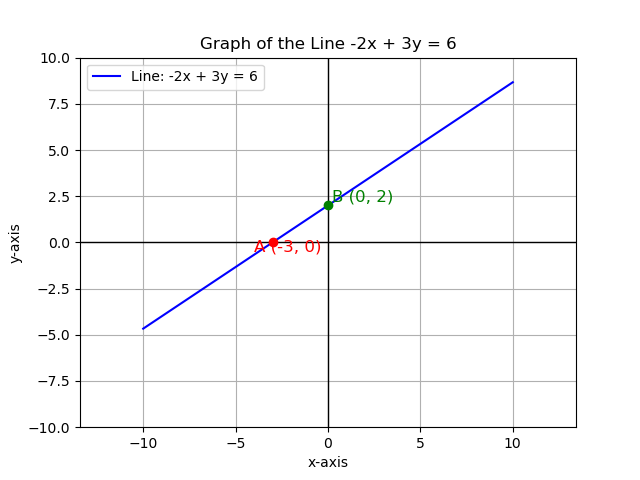
\includegraphics[width=\columnwidth, height=0.8\textheight, keepaspectratio]{figs/Figure_6.png}       
\end{align}
\end{document}